En este parte del proyecto se aborda la estructura establecida por Osterwalder Yves en el escrito “Generación de modelos de negocios”\cite{modeloNegocio}, se usa para tratar todas condiciones y requisitos fundamentales en el desarrollo de plan de negocios. 

Las fases y actividades establecidas se distribuyen de la siguiente manera:
\subsubsection{Fase 1: Presentación y compromiso del equipo}


\begin{itemize}
    \item Formación del grupo base.
    \item Formación del grupo de trabajo definitivo.
    \item Identificación de áreas de análisis
    \item Presentación del proyecto, procesos y metodologías.
    \item Documento de presentación aprobado (Anteproyecto).
\end{itemize}

En el cuadro \ref{Fase1} se establecen los objetivos de la fase asociada con la presentación y compromiso del equipo de manera que se puedan proyectar ciertos resultados esperados a través de unas actividades especificas de la fase.

\begin{adjustbox}{
            center,
             caption=[{Descripción de la fase 1}]{\centering Descripción de la fase 1. Fuente: : Autores.},
            label={Fase1},
            nofloat=table, vspace={20px}}
            \resizebox{\textwidth}{!}{
            \begin{tabular}{|c|c|c|c|}
            \hline
            \rowcolor[HTML]{D9EAD3} 
            \multicolumn{1}{|l|}{\cellcolor[HTML]{D9EAD3}\textbf{Fase 1}} &
            \multicolumn{1}{l|}{\cellcolor[HTML]{D9EAD3}\textbf{Objetivos Especificos}} &
            \multicolumn{1}{l|}{\cellcolor[HTML]{D9EAD3}\textbf{Actividades}} &
            \multicolumn{1}{l|}{\cellcolor[HTML]{D9EAD3}\textbf{Resultados Esperados}} \\ \hline
             &  & Conformación del equipo       & \begin{tabular}[c]{@{}c@{}}Tener claro el papel de cada uno\\  de los integrantes del equipo\end{tabular} \\ \cline{3-4} 
            &  & Búsqueda inicial de literatura & Análisis del contexto                                                                                      \\ \cline{3-4} 
        \multirow{-4}{*}{\begin{tabular}[c]{@{}c@{}}Presentación y \\ compromiso del \\ equipo\end{tabular}} &
        \multirow{-4}{*}{\begin{tabular}[c]{@{}c@{}}Dar a conocer los integrantes del equipo\\  e iniciar con el análisis de la situación,\\ planteamiento del problema\\  y proyectarnos trabajando de la mano.\end{tabular}} &
            Definir el planteamiento del problema &
            Definición precisa del problema \\ \hline
            \end{tabular}
            }

        \end{adjustbox}

\subsubsection{Fase 2: Análisis de la situación}
\begin{itemize}
    \item Identificación de la oportunidad de negocio, definición del producto o servicios.
    \item Estudio de mercado.
    \item Análisis de riesgos.
\end{itemize}

En el cuadro \ref{Fase2} se establecen los objetivos de la fase asociada al análisis de la situación de manera que se puedan proyectar ciertos resultados esperados a través de unas actividades especificas de la fase.

\begin{adjustbox}{
            center,
             caption=[{Descripción de la fase 2}]{\centering Descripción de la fase 2. Fuente: : Autores.},
            label={Fase2},
            nofloat=table, vspace={20px}}
            \resizebox{\textwidth}{!}{
            \begin{tabular}{|c|c|c|c|}
\hline
\rowcolor[HTML]{D9EAD3} 
\textbf{Fase 2} &
  \textbf{Objetivos Especificos} &
  \textbf{Actividades} &
  \textbf{Resultados Esperados} \\ \hline
 &
   &
  \begin{tabular}[c]{@{}c@{}}Definir el funcionamiento del\\ mercado de contratacion de personal IT\end{tabular} &
  \begin{tabular}[c]{@{}c@{}}Definición de producto\\  y posibles riesgos\end{tabular} \\ \cline{3-4} 
 &
   &
  Establecer las asociaciones claves &
  Modelo de negocio \\ \cline{3-4} 
 &
   &
   &
  Propuesta de valor \\ \cline{4-4} 
\multirow{-5}{*}{\begin{tabular}[c]{@{}c@{}}Análisis de la \\ situación actual\end{tabular}} &
  \multirow{-5}{*}{\begin{tabular}[c]{@{}c@{}}Realizar un análisis de mercado para\\ definir la factibilidad de creación \\ del producto para la gestion \\ de contratacion de personal IT\end{tabular}} &
  \multirow{-2}{*}{\begin{tabular}[c]{@{}c@{}}Efectuar la estructura \\ de costos\end{tabular}} &
  Estudio de mercado \\ \hline
\end{tabular}
            }

        \end{adjustbox}

\subsubsection{Fase 3: Definición de la empresa}
\begin{itemize}
    \item Identificación de la misión, la visión y el objeto de la empresa.
    \item Modelo de negocio que se abordará.
    \item Estructura organizacional y administrativa
    \item Tipo de sociedad a crear.
\end{itemize}
En el cuadro \ref{Fase3} se establecen los objetivos de la fase asociada con la definición del problema de manera que se puedan proyectar ciertos resultados esperados a través de unas actividades especificas de la fase.
\begin{adjustbox}{
            center,
             caption=[{Descripción de la fase 3}]{\centering Descripción de la fase 3. Fuente: : Autores.},
            label={Fase3},
            nofloat=table, , vspace={20px}}
            \resizebox{\textwidth}{!}{
            \begin{tabular}{|c|c|c|c|}
\hline
\rowcolor[HTML]{D9EAD3} 
\textbf{Fase 3} & \textbf{Objetivos Especificos} & \textbf{Actividades} & \textbf{Resultados Esperados} \\ \hline
                &                                & Definir Misión       &                               \\ \cline{3-3}
                &                                & Definir Visión       &                               \\ \cline{3-3}
                &                                &                      &                               \\
\multirow{-4}{*}{\begin{tabular}[c]{@{}c@{}}Definición de \\ la empresa\end{tabular}} &
  \multirow{-4}{*}{\begin{tabular}[c]{@{}c@{}}Establecer la misión y visión de la\\ empresa al igual que el ecosistema empresarial\end{tabular}} &
  \multirow{-2}{*}{Trazar los valores empresariales} &
  \multirow{-4}{*}{\begin{tabular}[c]{@{}c@{}}Conformación de la\\ \\ empresa con todos sus agregados y sus valores\end{tabular}} \\ \hline
\end{tabular}
            }

        \end{adjustbox}

\subsubsection{Fase 4: Estructuración}
\begin{itemize}
    \item Identificación de debilidades y fortalezas (Análisis interno).
    \item Identificación de las oportunidades y amenazas (Análisis externo).
    \item Identificación de funciones y procesos de negocio de la empresa.
    \item Ingeniería.
    \item Estudio técnico.
    \item Estudio legal.
    \item Plan financiero.
    \item Prototipo
\end{itemize}
En el cuadro \ref{Fase4} se establecen los objetivos de la fase asociada con la estructuración de manera que se puedan proyectar ciertos resultados esperados a través de unas actividades especificas de la fase.
\begin{adjustbox}{
            center,
             caption=[{Descripción de la fase 4}]{\centering Descripción de la fase 4. Fuente: : Autores.},
            label={Fase4},
            nofloat=table, vspace={20px}}
            \resizebox{\textwidth}{!}{
            \begin{tabular}{|c|c|c|c|}
\hline
\rowcolor[HTML]{D9EAD3} 
\textbf{Fase 4} & \textbf{Objetivos Especificos} & \textbf{Actividades}                          & \textbf{Resultados Esperados}     \\ \hline
                &                                & Definir presupuesto                           &                                   \\ \cline{3-3}
                &                                & Definir inversión inicial, ingresos y egresos & \multirow{-2}{*}{Estudio técnico} \\ \cline{3-4} 
                &                                & Definir naturaleza jurídica                   &                                   \\ \cline{3-3}
 &
  \multirow{-4}{*}{\begin{tabular}[c]{@{}c@{}}Definir estructura\\ legal del producto\end{tabular}} &
  Establecer propiedad intelectual &
   \\ \cline{2-3}
                &                                & Identificar obligaciones legales              & \multirow{-3}{*}{Estudio legal}   \\ \cline{3-4} 
                &                                & Realizar balance general                      &                                   \\ \cline{3-3}
                &                                & Definir un punto de equilibrio                &                                   \\ \cline{3-3}
                &                                & Análisis de indicadores financieros           &                                   \\ \cline{3-3}
                &                                & Realizar flujo de caja                        & \multirow{-4}{*}{Plan financiero} \\ \cline{3-4} 
                &                                & Realizar estudio del entorno                  &                                   \\ \cline{3-3}
\multirow{-11}{*}{Estructuración} &
  \multirow{-7}{*}{\begin{tabular}[c]{@{}c@{}}Realizar ingenieria \\ del proyecto\end{tabular}} &
  Realizar estado de resultados &
  \multirow{-2}{*}{Estudio ambiental} \\ \hline
\end{tabular}
            }

\end{adjustbox}

\subsection{Cronograma}

Se opta para construir el siguiente cronograma que tiene las actividades propuestas a realizar para el desarrollo exitoso de este proyecto y los tiempos en los que deben llevarse a cabo.

\begin{adjustbox}{
    center,
    caption=[{Cronograma de actividades}]{\centering Cronograma de actividades Fuente: Autores},
    label={Cronograma},
    nofloat=figure, vspace={7px}}


    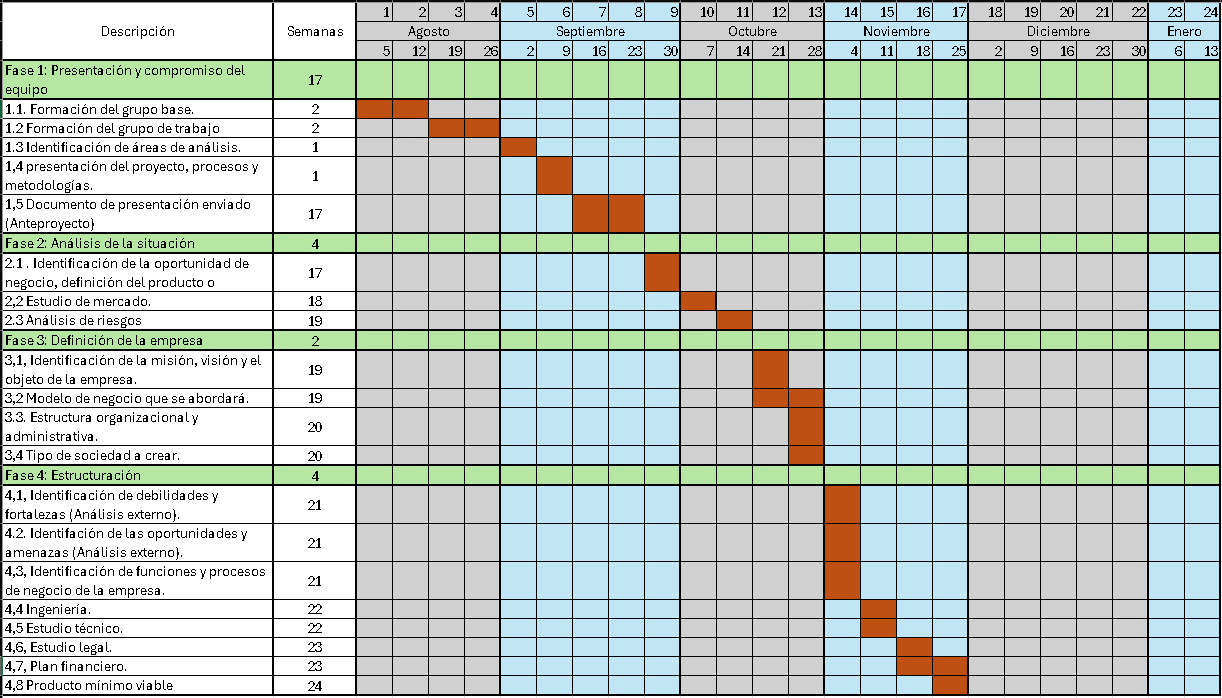
\includegraphics[width=1\textwidth]{Content/Images/cronogramaEmpre.PNG}
\end{adjustbox}



